\documentclass[11pt]{article}

\usepackage{a4wide}
\usepackage{mathptm}
\usepackage{xspace}
\usepackage{amsmath}
\usepackage{graphicx}
\usepackage{algorithm}
\usepackage{algpseudocode}
\usepackage{tikz}
\usepackage{tkz-graph}
\usetikzlibrary{shapes.misc, positioning}
\usepackage{listings}
\usepackage{color}
\usepackage{xcolor}

\definecolor{dkgreen}{rgb}{0,0.6,0}
\definecolor{gray}{rgb}{0.5,0.5,0.5}
\definecolor{mauve}{rgb}{0.58,0,0.82}

\lstset{frame=tb,
  language=Java,
  aboveskip=3mm,
  belowskip=3mm,
  showstringspaces=false,
  columns=flexible,
  basicstyle={\small\ttfamily},
  numbers=left,
  numberstyle=\tiny\color{gray},
  keywordstyle=\color{blue},
  commentstyle=\color{dkgreen},
  stringstyle=\color{mauve},
  breaklines=true,
  breakatwhitespace=true,
  tabsize=3
}
\begin{document}

\title{Report SpringApp Project Group 4}

\author{Jacek Antoni Wegrzynowski, Rashaad Wells Iversen, Veronicha C. T. Pettersen }

\maketitle

\begin{abstract}

\textcolor{red}{ 10-15 lines with the software technology and the highlights from the project that has been undertaken. }

This document describes the journey of a group of students at Western Norway University of Applied Sciences took to develop a web-based application prototype to create poll and receive votes.  The prototype's creation involved a new learned technology stack, integrating Angular, Spring Boot, JPA, Hibernate, H2, MQTT and Java.  We achieved significant functionalities, including user registration and authentication, poll and question creation, poll searching, and versatile voting mechanisms via both web interface and IoT integration.  Remarkably, these milestones were reached despite the team's initial lack of Java expertise, demonstrating a commendable learning curve and adaptability.  The successful implementation of these features showcases the prototype's potential to deliver a final product for polling.  While the complexity of our work may not align with every expectation, we take considerable pride in the achievements we have realized.  Our efforts reflect significant dedication and learning, particularly in areas initially unfamiliar to us.

\end{abstract}

%\input{commands}

\section{Introduction}
\label{sec:introduction}

Approximately 1 page on:


\begin{itemize}

\item \textcolor{red}{A brief introduction to the prototype implementation and topic of the project.}
In this project, an IoT-cloud software system has been developed. The system takes feedback from users in the form of yes/no votes on polls. The polls can be voted on either via an web interface or via an IoT-device. 

\item \textcolor{red}{Discuss (briefly) the technology stack that has been selected, mention related technologies (if relevant), primary arguments for choice of technology stack.}

Here we can maybe add an illustration from the powerpoint 


\item \textcolor{red}{A brief account of the results that have been obtained in the project.}

\item\textcolor{red}{ A one paragraph overview at the end, explaining how the rest of the report is / has been organised}

\end{itemize}

\noindent
This rest of this report is organised as follows:
Section~\ref{sec:technology} gives an ....


\section{Software Technology Stack}
\label{sec:technology}

\textcolor{red}{Introduce in (sufficient) depth the key concepts and architecture of the chosen software technologies. As part if this, you may consider using a running example to introduce the technology.}

\textcolor{red}{Emphasize the “new” software technologies that was selected by the group and which has not been covered in the course.}

\textcolor{red}{This part and other parts of the report probably needs to refer to
figures. Figure~\ref{fig:framework} from \cite{brown:96} just
illustrates how figure can be included in the report.}

Angular:
The front-end of the FeedApp is developed using Angular. Angular is a widely used framework that is used for building single-page applications (SPAs).

Fundamental Consepts of Angular: 
\begin{description}
\item[Components and Views]: The angular application is built upon components. For every component, there is a HTML template for the content of the web interface and a TypeScript class that controls the logic. The components are what defines the views, which is what  is displayed to the user on the webpage. 
\item[Dependency Injection (DI)]: Angular´s dependency injection (DI) system provides services to components. Services are classes that can contain business logic, data handling and functionalities that can be useful in multiple components. In our FeedApp implementation, we created services dedicated to managing authentication and handling poll data. These services made it possible to streamline data interactions and logic across different components, making it easier to control that the underlying operations and management of the data were handled consistently. 
\item[Routing]: The Angular Router handles the navigation between different views as users performs different tasks. This is a key element in SPAs since instead of reloading the page

Resourses used for writing this paragraph: https://angular.io/guide/architecture 
\end{description}

Spring Boot 

JSON Web Tokens 

H2, Hibernate 

Java Persistence API 

Mosquitto MQTT

\begin{figure}
  \centering
  \includegraphics[scale=0.5]{figs/framework.png}
  \caption{Software technology evaluation framework.}
  \label{fig:framework}
\end{figure}


\clearpage
\section{Design of the FeedApp Prototype}
\label{sec:design}

\subsection{Architectural Overview} 

Our fundamental idea of the FeedApp application was to mimic some of the Kahoot application capabilities while remaining simplistic, keeping alignment with good practices in software development and prototyping.  Our archtiecutre aims to meet requirements, demonstrate core functionality, and balance the effort put into development of a prototype.  \\

\noindent The application is accessible through web browsers, ensuring compatibility with devices such as smartphones, tablets, and computers.  Key features of the FeedApp are listed below:

\textcolor{red}{(rewrite so that each point is described in a full sentence)}

\begin{enumerate}
\item Ability to create and particpate in polls
\item Flexibility to cast votes via an IoT device or a web browser. 
\item Real-time display of voting results and analytics.
\item Third Party access to data for analytics
\item User Authentication
\end{enumerate}

\subsection{Domain Model} 

Our domain model of the FeedApp, is represented in a Unified Modeling Language (UML) class diagram representing the fundamental objects and their relationships. By doing this we describe  behavior and functions in a clear way so that we are all on the same page.  Throughout the development lifecycle of the FeedApp, this domain model has undergone iterative modifications. These adaptations were essential to maintain alignment with changes made in our objectives.  A primary focus during these modifications has been the preservation of simplicity within the system's architecture. By continuously refining the domain model, we have ensured that the FeedApp remains functionally efficient.

\subsubsection{Users}
The domain model describes an entity of a user and categorizes it into two distinct types based on account registration status.  Users with registered accounts are granted full access within the FeedApp including the capability to create and participate in both public and private polls.  This category of user must undergo an authentication process which is described in TODO:Section.  Users without registerd accounts are only allowed to participate in publicly accessible  polls.  This restriction is a delibarate choice, allwoing our development efforts to maintain simpliciy in implementation.  

\subsubsection{Polls}
A key feature of the system is the poll entity, characterized by distinct attributes such as a title, an identification number, and the option to be set as private or public. Each poll is required to have a time limit and are also designed to integrate with Internet of Things (IoT) devices.  Furthermore, polls are designed to be flexible, allowing an unrestricted number of questions. The application does not impose a limit on the quantity of questions per poll.  In addition to this, for private polls, there is a feature to specify a list of authorized users who are permitted to vote. 
In the design of polls, the questions must be structured as binary-choice and closed-ended.  This format restricts responses to one of two predetermined options, exemplified by pairs such as True/False, Yes/No, or Pancakes/Waffles.  While the application does not impose time limits on individual questions, it integrates time restrictions at the poll level.  This design choice, made for ensuring simplicity in implementation, focuses on the entire poll rather than individual questions.

\subsubsection{IOTDevice}
For this project, a physical IoT device was chosen to add the interactive dimension to the polling process.  This device is intentionally simplistic, capable only of transmitting voting data without knowledge of the specific poll or question involved.  It operates via a Mosquitto broker, which relays messages from the IoT device to the feed application. The integration with the IoT device is minimalistic. The device's primary function is to acknowledge a voting action and communicate this to the feed application. It is not equipped to discern details about the poll or the voting options. The absence of an on-device display is compensated for by using a command-line interface to indicate when a vote has been cast. This setup was demonstrated in the submitted video, showcasing the Mosquitto broker's role in facilitating communication between the IoT device and the feed application.

\subsubsection{IOTDisplay}
The project's infrastructure includes an Internet of Things (IoT) device, functioning independently on a dedicated hardware platform. This device establishes a wireless connection with a Windows-based HP laptop, which serves a dual purpose: as a control unit and as a display for the IoT device's operations. The design stipulates that both the IoT device and the laptop must share the same Wi-Fi network for seamless communication.

\subsubsection{IOTDevice Integration with FeedApp}
Further enhancing the system's architecture is the incorporation of a Linux virtual machine (VM) on the HP laptop. This VM is designated as the application server, managing the core functionalities of the feedback feed application. Notably, the VM's connectivity is not restricted to the same Wi-Fi network as the IoT device, offering flexibility in network configurations. It communicates with the IoT device through a Mosquitto broker, which acts as an intermediary in message transmission. The IP address of the Mosquitto broker is hardcoded into the system for consistent connectivity.

The application leverages a REST API to handle incoming data from the IoT device. When a user interacts with the IoT device, such as by pressing a button, this action triggers a message that is relayed by the Mosquitto broker to the feed application. The application's REST API is configured to recognize this input, determining the active poll and the specific question being addressed by the IoT device. While the mechanism for transitioning between different poll questions was not fully established, the conceptual framework suggests that the REST API would facilitate this progression by incrementally recording votes and navigating to subsequent questions.

\subsubsection{Analytics}
Once the a vote is cast on the last quesiton in the poll, the application is designed to immediately reflect the analytical data offering insight into collective responses.  The system is designed to facilitate the display of analytics for all polls, regardless of their current status (active or inactive).  This functionality is implemented through a standardized display template, which is accessible via web browsers. The template ensures uniformity in the visualization of analytics, providing a coherent and consistent user experience. In addtion, the system's architecture allows for third-party applications to access poll-related data.  This capability enables external entities to conduct their own analytical assessments.  However, it is important to note that the scope of data accessible to third-party applications is confined to poll-level information. Granular data pertaining to individual questions within the polls is not available for external analysis.

\subsection{FrontEnd Design} 
To get an overview of how we wanted to implement the user interface, an application flow diagram was modeled. 
The diagram displays how the user navigates through the different frames in the front end of the application:

\begin{figure}[h]
  \centering
  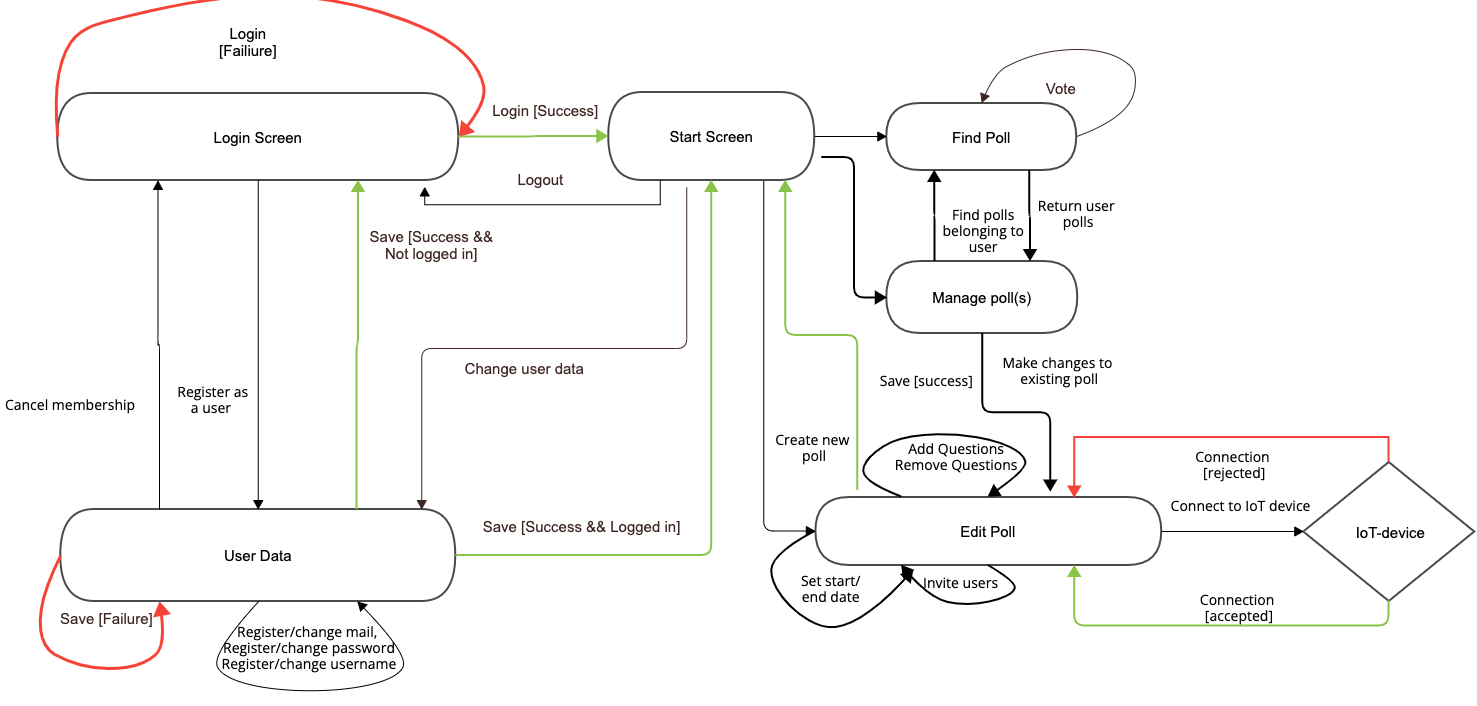
\includegraphics[scale=0.30]{figs/Application Flow Diagram (1).png}
  \caption{Application Flow Diagram}
  \label{fig:appFlow}
\end{figure}

Each screen has in the diagram been modelled as a state, and for every state, the user is able to do some action or provide some input. 
These actions or inputs are modelled as transitions, and are in the figure above illustrated with arrows. Transitions that results in errors are 
colored red, and transitions that does not result in errors are colored green. Our application consists of six screens. We have a login screen, 
where the user can either login, or create a new user. Once the user is logged in, he is directed to a start screen, where he gets the option to 
do multiple actions. He can search for a poll, which then can be voted on, or he can view and manage his own polls. He can create new polls,
and in this state he gets the option to pair the poll with an IoT device. 

The example below shows how you may include code. There are similar
styles for many other langages - in case you do not use Java in your
project. You can wrap the listing into a figure in case you need to
refer to it. How to create a figure was shown in Section~\ref{sec:technology}.

\lstinputlisting[language=java]{code/BoksVolum.java}

\section{Prototype Implementation}
\label{sec:implementation}

\subsection{Frontend}
The following components has been implemented for the front end:

\begin{itemize}
	\item Login: this is the first view that the user are presented with. It’s main purpose is to
authenticate users, and help them access the application. It contains input fields for
username and password. When the user presses “Log in”, he is taken to the main-page of the
application. If the user is not registered, he can easily do so by pressing the “Register”-
button.
	\item Register: here the user is presented a schema, where he can register and that way access the
application. He needs to add an email address, a username and a password. Once the
information is submitted, the user is sent back to the login page.
	\item Main-page: This component contains buttons that lets the user easily navigate to all parts of
the application quickly.
	\item Find-poll: Here the user can search for a poll via its id, or by a poll-name. All the polls that
matches the input will then be displayed with the option to vote on it.
	\item Create-poll: Here the user can create a new poll. He can decide the questions that should be
displayed, when the poll is active, if it is private and invite users to participate in it. Once
created, a poll-id is given to the user. This can for example be given to other users and used
to search for the poll.
	\item Vote: Here the user gets to submit votes to active polls.
\end{itemize}

A authentication service, a poll service and a voting service has also been created to handle logic that
can be applied to multiple components. The authentication service handles operations such as
logging the user in to the application and searching for users. The poll service handles logic depicting
the polls such as finding polls, creating polls and changing polls. The Voting service handles the logic
connected to the voting.

There are also a few features that we modelled into our application in the first phase of this project,
but due to the time constraints are yet to be implemented. These include Poll management and User
management. Currently the application allows users to create and participate in polls. However, the
management of the polls is not yet functional. The same goes for the management of the user
settings. The buttons has been created in the main-page component, but they are not directing the
users to new views yet.

\input{sections/evaluation}

\clearpage
\section{Conclusions}

\textcolor{red}{Concludes on the project, including the technology, its maturity, learning curve, and quality of the documentation.}

\textcolor{red}{The references used throughput the report should constitute a well chosen set of references, suitable for someone interesting in learning about the technology.}\\



\noindent The overall design framework for the FeedApp project was pre-established at the beginning of the assignment. This design was further amplified through the course of various lectures that looked into different aspects of the project.  Given our initial unfamiliarity with many of the technologies outlined in the project's scope, we proceeded to adopt those specified in the project guidelines.\\

\noindent The project's brief did offer the option to incorporate one additional technology, which, while seemingly providing a degree of flexibility, also imposed certain constraints on our technological explorations. For example, questions such as the feasibility of implementing the project in Python, the existence of a Python persistence model, or Python's capability to interface effectively with a database, remained unexplored. These potential avenues of inquiry could have provided a valabue alternative allowong a more complex design and quicker development approach.\\

\noindent However, the intensive and time-consuming nature of the assignments precluded a thorough investigation into these alternative technological possibilities. As a result, the project proceeded within the confines of the pre-specified technology stack, leaving some questions about potential alternative implementations and technologies unanswered.

\bibliographystyle{plain}
\bibliography{report.bib}{}

\end{document}
